\documentclass{tufte-handout}

%\geometry{showframe}% for debugging purposes -- displays the margins

\usepackage{amsmath}

% Set up the images/graphics package
\usepackage{graphicx}
\setkeys{Gin}{width=\linewidth,totalheight=\textheight,keepaspectratio}
\graphicspath{{graphics/}}

\title{Lipid Digestion and Absorption}
\author{}
\date{}  % if the \date{} command is left out, the current date will be used

% The following package makes prettier tables.  We're all about the bling!
\usepackage{booktabs}

% The units package provides nice, non-stacked fractions and better spacing
% for units.
\usepackage{units}

% The fancyvrb package lets us customize the formatting of verbatim
% environments.  We use a slightly smaller font.
\usepackage{fancyvrb}
\fvset{fontsize=\normalsize}

% Small sections of multiple columns
\usepackage{multicol}

% Provides paragraphs of dummy text
\usepackage{lipsum}

% These commands are used to pretty-print LaTeX commands
\newcommand{\doccmd}[1]{\texttt{\textbackslash#1}}% command name -- adds backslash automatically
\newcommand{\docopt}[1]{\ensuremath{\langle}\textrm{\textit{#1}}\ensuremath{\rangle}}% optional command argument
\newcommand{\docarg}[1]{\textrm{\textit{#1}}}% (required) command argument
\newenvironment{docspec}{\begin{quote}\noindent}{\end{quote}}% command specification environment
\newcommand{\docenv}[1]{\textsf{#1}}% environment name
\newcommand{\docpkg}[1]{\texttt{#1}}% package name
\newcommand{\doccls}[1]{\texttt{#1}}% document class name
\newcommand{\docclsopt}[1]{\texttt{#1}}% document class option name

\begin{document}

\maketitle% this prints the handout title, author, and date

\begin{abstract}
\noindent This unit will cover the digestion and absorption of lipids, and the generation of chylomicrons.  Lipid digestion is quite a bit different from the soluble digestion of carbohydrates and lipids, so we will also cover bile acids and their role in absorption.  Chapter 15 in Lippincott's Illustrated Reviews in Biochemistry available in reserve\cite{Ferrier2017}.
\end{abstract}

\tableofcontents

\pagebreak
\section{Learning Objectives}

\begin{itemize}
\item Identify the roles of Lingual Lipase, Gastric Lipase and Pancreatic Lipase including their locations and specific roles on lipid digestion in the stomach
\item Understand the role of bile salts in the formation of micelles, and explain how diseases of bile formation can affect an individual
\item Explain the transport mechanisms of lipids across the apical and basolateral membranes, and how they differ between lipid classes
\item Describe the re-esterification processes in the enterocyte
\item Explain the nature, formation and fate of the chylomicron and its role in lipid transportation
\end{itemize}

\section{Key Vocabulary and Concepts}
\begin{itemize}
	\item Micelle
	\item Lipases and Colipase
	\item CCK and Secretin 
	\item Gallbladder and Bile Synthesis
	\item Primary, Conjugated and Secondary Bile Salts
\end{itemize}

\section{Dietary Lipids and Dietary Intake}

The three main dietary lipids we ingest are triglycerides, phospholipids and cholesterol.  Of these, on average we consume much more in terms of triglycerides (95g for men, 65g/day for women) than phospholipids (1-2g/day) or cholesterol (300 mg/day).  For the average person that's about 1/3 of their total caloric intake \citep{NationalCenterforHealthStatistics2017}.  Dietary lipids are also our only source of the essential $\omega$3 and $\omega$6 fatty acids.  Furthermore several lipid soluble vitamins are carried and absorbed along with lipids.  These include vitamins A, D, E and K, so impairments in lipid absorption can affect their absorption as well.

\section{Lipid Digestion in the Upper Digestive Tract}

There is substantial debate about whether lipids can be tasted, in the way that we have specific receptors in our tongue that can sense sweet, bitter, sour, salt, and umami flavors.  While there are fatty acid receptors on the tongue, at this stage most lipids are in the triglyceride form.  Rather lipid flavor is thought to be a combination of several fatty acid receptors, along with the mechanical sensation of lipids in the oral cavity \citep{DiPatrizio2014}.

Lipid digestion, relative to carbohydrate digestion is relatively simple from an enzymatic perspective.  This process is somewhat complicated by the insoluble nature of fat.  Rather than letting food diffuse and break down into aqueous pieces, fat will aggregate in globules and often float as it passes through the digestive tract\sidenote{Think about how oil separates in water.}.  Therefore lipid digestion is a combination of enzymatic processing, along with the solubilization needed for absorption.

\newthought{The first lipid digestive enzymes are secreted in the oral cavity.}  This enzyme is known as \emph{Lingual Lipase} and is secreted from glands underneath the tongue.  While it is present in the mouth, it is only functional in the low pH environment, such as that in the stomach.  Lingual Lipase tends to cleave the sn3 fatty acids from triglycerides\sidenote{Recall, phospholipids do not have a fatty acid esterified at the sn3 position, that is where the headgroup is located.}.  This results in a diacylglycerol and a free fatty acid. Lingual Lipase is especially effective in removing medium chain fatty acids from triglyceride molecules \citep{Jensen1983}.

\newthought{Gastric Lipase also functions in the stomach.}  This enzyme is secreted from chief cells in the stomach, and like Lingual Lipase is most active in the low pH of the stomach\sidenote{Though it is able to continue functioning into the small intestine.}.  Gastric Lipase prefers to release fatty acids from the sn1 and sn3 positions of a lipid.  For both phospholipids and triglycerides this leaves a monoacylglycerol with the fatty acid still in the sn2 position.  The removal of the acyl chain make the lipid much more soluble and easier to emulsify into smaller droplets.

\newthought{The process of emulsification is essential to lipid absorption.}  Emulsification is the breaking of lipid droplets in to smaller and smaller particles.  A large globule of fat is not going to be able to easily pass through a cellular membrane, so as lipids pass through the digestive tract, both enzymatic digestion and mechanical churning to make the droplets as small as possible.

\section{Absorption and Digestion of Lipids in the Small Intestine}

Most lipid digestion and absorption\sidenote{In most cases greater than 90\%.} occurs within the small intestine.  At this point the semi-digested, emulsified lipid droplets come into contact with bile salts, which further aid in their solubilization into very tiny lipid droplets called micelles.  Micelles are generally coated with an amphipathic layer of bile salts, and contain an internal core of fatty acids, and monoacylglycerols.

\subsection{Bile Salts and Their Regulation}

Bile salts are cholesterol-derived compounds that are generated initially in the liver\sidenote{We will discuss this in the lipid transport and synthesis lectures, but cholesterol is generally made throughout the body, with excess trafficked to the liver.  Since it cannot be used for fuel, cholesterol is \emph{only} released in the form of bile acid secretion.}  In the liver through a series of enzymatic steps, cholesterol is converted into \emph{primary bile acids} such as cholic acid and chenodeoxycholic acid.  This step is rate-limited by an enzyme known as 7-$\alpha$-hydroxylase, which in turn is transcriptionally downregulated when liver primary bile acids are high \citep{Ramirez1994}\sidenote{The sensing of bile acids turns out to be an emerging area of research.  The actual receptors for bile acids are a transcription factor known as FXR (farnesoid-x-receptor) and a receptor on the cellular surface known as TGR5.  For 7-$\alpha$-hydroxylase, FXR seems to be the more important regulator \citep{Sinal2000}.}.

\newthought{Conjugated bile acids\sidenote{A third class of bile acids, known as secondary bile acids are generated in the large intestine by bacterial modification of secreted bile acids.  Since these are reabsorbed and sent back the liver, the secondary bile acids, known as deoxycholic acid and lithocholic acid can then also be conjugated in the liver.  Secondary bile acids comprise of about 20-40\% of the total bile acid pool.  Interestingly changes in bile acids are thought to play a role in the metabolic benefits of bariatric surgery \citep{Evers2017a}.} are generated from primary bile acids.}  while still in the liver, bile acids have either a glycine or a taurine\sidenote{Taurine is an amino acid, derived from cysteine that is not used in proteins.} amino acid group added to them.  This yields a conjugated bile acid, of which there are several species.  This new bile acid is very amphipathic, with a charged group from the amino acid on one end and the modified cholesterol on the other end.  This makes bile acids very effective in interacting with and solubilizing dietary lipids.

\newthought{Bile salts are efficiently reabsorbed}, after their lipid cargo has been absorbed with up to 95\% of bile salts being reabsorbed via a sodium co-transporter in the terminal illeum.  One approach therefore to remove cholesterol from the blood stream is bile acid sequestrants that impair the uptake of bile salts, and thus the release of cholesterol.

\subsection{Uptake of Lipids in the Small Intestine}

After a brief diversion about bile salts and their role in generating lipid micelles lets return to the small intestine where we now have partially hydrolyzed triglycerides and phospholipids.  A third Lipase, called \emph{Pancreatic Lipase} is secreted into the small intestine, it again is specific to the sn1/sn3 positions but compared to Lingual Lipase, has stronger activity towards long chain fatty acids \citep{Jensen1983}.  Pancreatic Lipase activity is dependent on a coenzyme called \emph{colipase}.  It is secreted as a precursor called procolipase, and is activated by trypsin-mediated cleavage\sidenote{This is common theme that will come up again in the protein digestion unit wherein trypsin is also secreted as an inactive precursor and is activated by cleavage by enteropeptidase.}.  Recall that at this stage many lipids are solubilized within bile-salt containing micelles.  The presence of colipase allows Pancreatic Lipase to be active even on lipids contained within the micelles.  More details about how colipase can help Pancreatic Lipase function can be found in \citet{VanTilbeurgh1999}.

\newthought{Cholesterol and Phospholipids are also digested in the small intestine.}  We have been focusing mainly on triglycerides, but two more enzymes in the small intestine are important for the absorption of phospholipids and cholesterol.  For phospholipids, the key enzyme is Pancreatic Phospholipase.  This is a class A2 phospholipase\sidenote{This means that it releases the fatty acid from the sn2 position of a phospholipid, leaving a fatty acid at the sn1 position, and the headgroup at the sn3 position.}.  At this stage the phospholipid is known as a lysophospholipid.  For cholesterol if the cholesterol is esterified\sidenote{Meaning it has a fatty acid conjugated to it.} this is removed by an enzyme termed Cholesterol Esterase.  Similarly to a lysophospholipid, cholesterol is now in a more amphipathic form allowing for better absorption.


\newthought{Cholesterol uptake is mediated by the NPC1L1 transporter.}  TThe predominant pathway for cholesterol uptake is via a steroid transporter called NPC1L1\sidenote{Niemann-Pick C1 Like 1, not the most useful name, it is based on homology with the lysosomal cholesterol transporter that causes Niemann-Pick disease, a disorder which involves lipid accumulation within lysosomes of cells.}\citep{Altmann2004,Iqbal2005}.  Plant sterols, which look very similar to cholesterol are imported along with cholesterol, but then are specifically exported back into the gut lumen via ATP-dependent transporters ABCG5/8\sidenote{Why do you think this step requires active transport?}.  Cholesterol uptake is reduced when enterocyte cholesterol levels are high. For example, bile acid synthesis deficiency\sidenote{Such as mutations in 7-$\alpha$-hydroxylase,  prevents bile acid production and secretion.} results in a dramatic decrease in cholesterol absorption to balance the limited release \citep{Repa2000,Wang2007d}.  The mechanism for this is via a transcription factor called SREBP2.  Normally SREBP2 increases the levels of NPC1L1.  When cholesterol levels are high, SREBP2 is inhibited, and cholesterol uptake is reduced (see Figure \ref{fig:srebp2}.  The upshot of this is that when endogenous cholesterol levels are high, dietary cholesterol absorption is reduced.  This is likely one reason why dietary cholesterol intake does not strongly modulate blood cholesterol levels.

\begin{marginfigure}
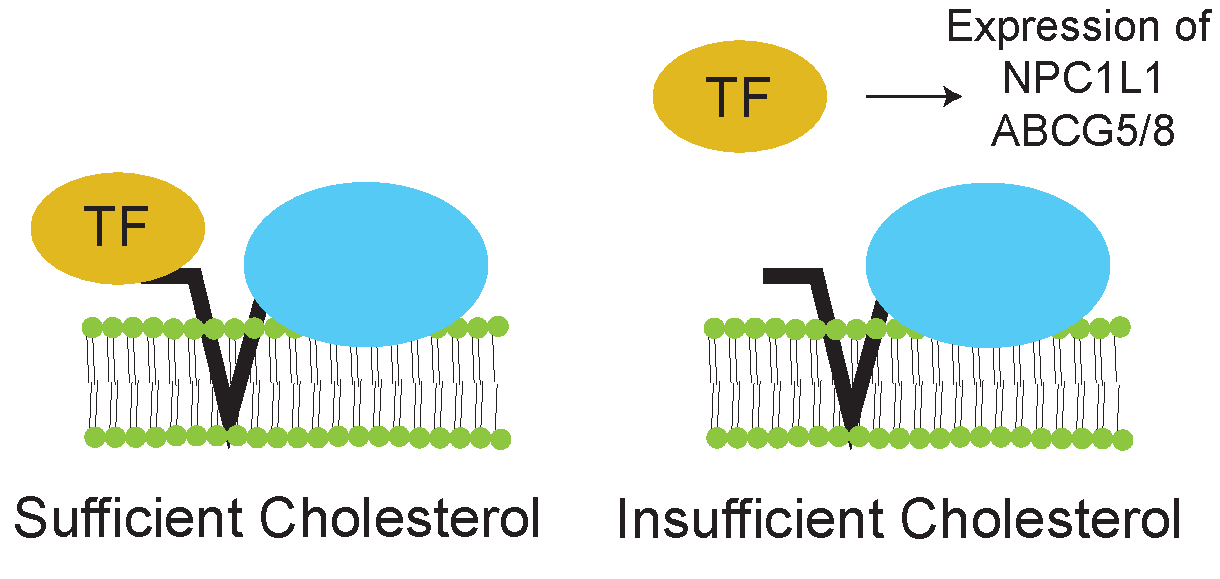
\includegraphics{figures/srebp2-intestine.pdf}
\caption{Regulation of SREBP2.  When there is insufficient cholesterol, SREBP2 is cleaved releasing the transcription factor (TF) fragment, where it can go to the nucleus and drive expression of cholesterol uptake genes such as \textit{NPC1L1}, \textit{ABCG5/8.}.  This means that at sufficient cholesterol levels absorption is largely reduced.}
\label{fig:srebp2}
\end{marginfigure}

\newthought{The remaining micelles contain fatty acids, monoacylglycerols\sidenote{With a fatty acid still in the sn2 position} and lysophospholipids.}  These lipids are absorbed across the apical membrane of enterocytes.  The precise mechanism seems to be a combination of passive transport and passive diffusion of micelles within the membranes, leaving the bile salts in the gut lumen.  Remember that both micelles and phospholipid membranes are very amphipathic, so one theory is that the lipid containing micelles just passively pass through the membrane.  Another thought is that they are bound to surface receptors then endocytosed\sidenote{This means that they are actively brought into the enterocyte via a biological import process}.  Either way, the majority of lipids are taken out of the gut lumen into the microvilli in the small intestine.


\subsection{Short Chain Fatty Acid Absorption}

Both short and medium chain fatty acids are more or less soluble in water and therefore do not require micelles for transport into the enterocytes.  These fatty acids are thought to be passively absorbed in the small intestine after digestion.

\newthought{Short chain fatty acids are derived from fiber.}  On the other hand, short chain fatty acids are more rare in our diet than long chain fatty acids\sidenote{These include things like acetate, butyrate and propionate}.  If ingested directly these can be absorbed by enterocytes, but most SCFA's are generated by our microbiome in the large intestine.  These bacteria use undigested fiber and unabsorbed proteins and peptides as fuel.  The major products of these reactions are SCFA \citep{Cummings1987}.  Colon epithelial cells can take up these metabolites, and use these SCFA as a fuel source, preferring butyrate.  Acetate and propionate to enter the circulation and enter the circulation.  While this may seem like a minor event, SCFA's provide about 10\% of our total caloric requirements and are a major way by which the gut microbiome can affect our energy balance.  For more details about SCFA and bacterial physiology refer to a recent review by \citet{Koh2016}.

\subsection{Endocrine Control of Lipid Digestion and Absorption}

We have mentioned several pancreatic and biliary secretions that aid in digestion of lipids.  The major regulators are cholecystokinin and secretin.  CCK is released from the lower duodenum and acts at several places including the gallbladder and pancreas.  In the gallbladder, CCK promotes contraction of the gallbladder, and relaxation of a sphincter connecting the bile duct to the duodenum\sidenote{This is known as the Sphincter of Oddi.}.  This results in excretion of bile salts into the small intestine.  As we have discussed previously CCK\sidenote{Secreted from enteroendocrine cells, also known as L-cells.}, is activated by the parasympathetic nervous system and inhibited by the sympathetic nervous system.  At the same time, CCK promotes the release of sodium bicarbonate and Pancreatic Lipase and colipase from the pancreas.  This process is also aided by secretin which also promotes pancreatic juice release.

\section{Transport of Lipids out of the Enterocytes}

Lipids are absborbed as free cholesterol, monoacylglycerol, lysophospholipids and free fatty acids into the enterocyte.  Each of these can be quite toxic to the cell, so they are very rapidly \emph{reconverted} into storage forms (esterified cholesterol and triglycerides).  This re-esterification is critically important for absorption and eventual transport to other tissues.

\newthought{Within enterocytes, the neutral lipids are packaged into large lipoprotein complexes called Chylomicrons.}  This is the first lipoprotein complex we will discuss.  These particles vary in size from quite large (like chylomicrons) to very small and dense\sidenote{The high density lipoproteins or HDL we be described in the lipid transport lecture.}  The surface of the chylomicrons contains phospholipids\sidenote{Mostly phosphatidylcholine \citep{Wood1964}.}, free cholesterol and specific amphipathic proteins called \emph{apolipoproteins}.  In the case of chylomicrons, these protein are Apolipoproteins A1 and B48.  The chylomicrons are secreted from the enterocytes into the lacteals of the lymphatic system.  They then bypass the portal vein at first and travel to peripheral sites for rapid utilization in tissues such as adipose and muscle.  Once in circulation, chylomicrons pick up Apolipoproteins CII and E.  As we will describe in the lipid transport lecture these allow for the chylomicrons to recognize and activate Lipoprotein Lipase for final delivery of fatty acids and cholesterol to peripheral tissues.  

\newthought{Medium and short chain fatty acids on the other hand,} are secreted directly into the bloodstream.  These more soluble fatty acids are directly transported via the portal vein to the liver,.  This is one of the reasons why gallbladder and chylomicron-generating diseases can be treated with medium chain fatty acids, and why medium chain fatty acids are rapidly converted into ketones.


\bibliography{library}
\bibliographystyle{plainnat}

\end{document}
